

\tikzset{every picture/.style={line width=0.75pt}} %set default line width to 0.75pt        

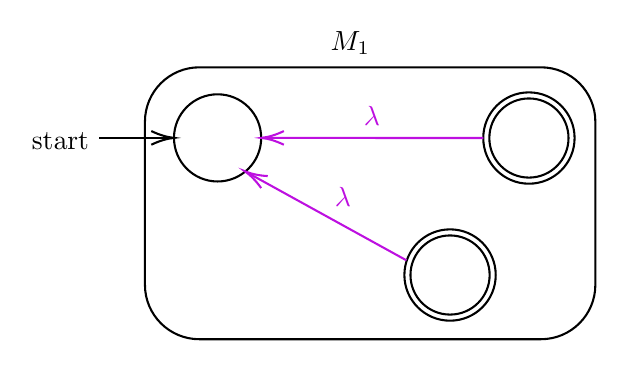
\begin{tikzpicture}[x=0.75pt,y=0.75pt,yscale=-1,xscale=1]
%uncomment if require: \path (0,300); %set diagram left start at 0, and has height of 300

%Straight Lines [id:da21164986404088237] 
\draw    (172,130) -- (206,130) ;
\draw [shift={(208,130)}, rotate = 180] [color={rgb, 255:red, 0; green, 0; blue, 0 }  ][line width=0.75]    (10.93,-3.29) .. controls (6.95,-1.4) and (3.31,-0.3) .. (0,0) .. controls (3.31,0.3) and (6.95,1.4) .. (10.93,3.29)   ;
%Shape: Circle [id:dp2758626329537419] 
\draw   (208,130) .. controls (208,118.4) and (217.4,109) .. (229,109) .. controls (240.6,109) and (250,118.4) .. (250,130) .. controls (250,141.6) and (240.6,151) .. (229,151) .. controls (217.4,151) and (208,141.6) .. (208,130) -- cycle ;
%Shape: Donut [id:dp11787073994627706] 
\draw   (359.93,130.07) .. controls (359.93,119.54) and (368.47,111) .. (379,111) .. controls (389.53,111) and (398.07,119.54) .. (398.07,130.07) .. controls (398.07,140.6) and (389.53,149.13) .. (379,149.13) .. controls (368.47,149.13) and (359.93,140.6) .. (359.93,130.07)(357,130.07) .. controls (357,117.92) and (366.85,108.07) .. (379,108.07) .. controls (391.15,108.07) and (401,117.92) .. (401,130.07) .. controls (401,142.22) and (391.15,152.07) .. (379,152.07) .. controls (366.85,152.07) and (357,142.22) .. (357,130.07) ;
%Rounded Rect [id:dp06917909208230033] 
\draw   (194,122.2) .. controls (194,107.73) and (205.73,96) .. (220.2,96) -- (384.8,96) .. controls (399.27,96) and (411,107.73) .. (411,122.2) -- (411,200.8) .. controls (411,215.27) and (399.27,227) .. (384.8,227) -- (220.2,227) .. controls (205.73,227) and (194,215.27) .. (194,200.8) -- cycle ;
%Shape: Donut [id:dp2430030625706079] 
\draw   (321.93,196.07) .. controls (321.93,185.54) and (330.47,177) .. (341,177) .. controls (351.53,177) and (360.07,185.54) .. (360.07,196.07) .. controls (360.07,206.6) and (351.53,215.13) .. (341,215.13) .. controls (330.47,215.13) and (321.93,206.6) .. (321.93,196.07)(319,196.07) .. controls (319,183.92) and (328.85,174.07) .. (341,174.07) .. controls (353.15,174.07) and (363,183.92) .. (363,196.07) .. controls (363,208.22) and (353.15,218.07) .. (341,218.07) .. controls (328.85,218.07) and (319,208.22) .. (319,196.07) ;
%Straight Lines [id:da844076689908255] 
\draw [color={rgb, 255:red, 189; green, 16; blue, 224 }  ,draw opacity=1 ]   (320,189) -- (243.75,146.97) ;
\draw [shift={(242,146)}, rotate = 388.87] [color={rgb, 255:red, 189; green, 16; blue, 224 }  ,draw opacity=1 ][line width=0.75]    (10.93,-3.29) .. controls (6.95,-1.4) and (3.31,-0.3) .. (0,0) .. controls (3.31,0.3) and (6.95,1.4) .. (10.93,3.29)   ;
%Straight Lines [id:da35533846506045697] 
\draw [color={rgb, 255:red, 189; green, 16; blue, 224 }  ,draw opacity=1 ]   (357,130.07) -- (252,130) ;
\draw [shift={(250,130)}, rotate = 360.03999999999996] [color={rgb, 255:red, 189; green, 16; blue, 224 }  ,draw opacity=1 ][line width=0.75]    (10.93,-3.29) .. controls (6.95,-1.4) and (3.31,-0.3) .. (0,0) .. controls (3.31,0.3) and (6.95,1.4) .. (10.93,3.29)   ;

% Text Node
\draw (138,126) node [anchor=north west][inner sep=0.75pt]   [align=left] {start};
% Text Node
\draw (282,77.4) node [anchor=north west][inner sep=0.75pt]    {$M_{1}$};
% Text Node
\draw (298,113.4) node [anchor=north west][inner sep=0.75pt]    {$\textcolor[rgb]{0.74,0.06,0.88}{\lambda }$};
% Text Node
\draw (284,152.4) node [anchor=north west][inner sep=0.75pt]    {$\textcolor[rgb]{0.74,0.06,0.88}{\lambda }$};


\end{tikzpicture}